% Introdu��o
\chapter{Introdução}


% TODO: Add more references
% TODO: Add Google Trend Big Data image


% In the last ten years, the search for terms such as big data, data analysis, and data visualization has increased enormously. There is a lot of reasons for this phenomenon, one of them is that with the computing power advancement we now have to deal with huge masses of data, which grows daily, from different sources in several formats in an incredibly short time. Therefore new challenges are rising in the data analysis field: How to process these immense quantities quickly and efficiently? How to visualize this amount of data? How to clean the dataset without losing important points?

Nos últimos dez anos, a busca por termos como \textit{big data}, análise de dados e visualização de dados tem aumentado notoriamente. Existem muitas razões para esse fenômeno, um deles é que com o avanço do poder computacional nós agora lidamos com imensas quantidades de dados, que crescem diariamente, de diversas fontes, em vários formatos e num incrível curto espaço de tempo. Dessa forma, novos desafios vêm surgindo na área de análise de dados: Como processar essas imensas quantidades rápida e eficientemente? Como visualizar esse montante de dados? Como \textit{limpar} o conjunto de dados sem perder pontos importantes?

% When it comes to the data analysis field and the analyst is working with large datasets, is very common to have a lot of points with attributes very distant from the rest of the dataset. This happens because when more huge is your dataset, more easily you can find abnormal points that will be more distant from the normal distribution. This kind of behavior is important to the analyst study and discover more information about the dataset itself and with this, he could take more accurate decisions and propose better statements. Usually, this concern about anomalous data was not too relevant for the most researches, but this behavior is changing since significant information can be discovered analyzing those uncommon points.

No que se refere ao campo da análise de dados e o analista está lidando com grandes \textit{datasets}, é muito comum encontrar vários pontos com atributos muito distantes do resto de seu conjunto. Isto acontece porque quanto maior é o \text{dataset}, mais facilmente se pode encontrar pontos atípicos que serão mais distantes da distribuição normal. Esse comportamento é importante ser estudado pelo analista para que seja descoberto mais informações sobre o dataset em si e com isso possa ser tomado decisões mais precisas e proposto melhores afirmações. Geralmente, essa preocupação sobre dados anômalos não era tão relevante para a maioria das pesquisas, mas isso vem mudando a partir de que informações importantes podem ser descobertas com essa análise de pontos incomuns.

% These specific data with those characteristics is called \textit{Outliers} and is very decisive that the current data analysts pay more attention to those data, because important information may be hidden inside these peculiar data.

Esse tipo específico de dado com essas características é chamado de Outliers e é muito importante que os atuais analistas de dados deem mais atenção para esses dados, pois informações importantes podem estar escondidas entre esses conjuntos particulares.

% For example, if we get an isolated dataset about NYC taxis from 2011 and analyze the frequency of requests at the entire year, it will appear a lot of points very distant from the average curve and this will indicate an unusual behavior in this collection. 

Por exemplo, se pegarmos um conjunto de dados isolado sobre os fluxo de táxis de Nova Iorque de 2011 e analisarmos a frequência de corridas no ano inteiro, irão aparecer muitos pontos fora dessa curva média e isso indicaria um comportamento anômalo nessa coleção.

% Generally, the first step to take in this situation is to remove the irregular points and continue the processing with the rest of the dataset, but if we get another isolated dataset about the wind speed from the same NYC region and compare this exactly space of time, we will perceive few peaks of high speed indicating hurricane at the same time \cite{DBLP:journals/debu/FreireCVZ16} as presented in Figure \ref{fig:freire-paper-taxy-wind}. Analyses like this prove the importance of detect, study and interpret those outliers to increase the knowledge obtained from this dataset.

Geralmente, a primeira tarefa a se fazer nessa situação era remover esses pontos irregulares e continuar o processamento com o resto do conjunto, mas se pegarmos outro conjunto de dados isolado sobre a velocidade do vento na região de Nova Iorque e no mesmo intervalo de tempo, nós iremos perceber algum picos de alta velocidade indicando furacões no mesmo momento e na mesma região da queda das corridas de táxi, como apresentado na Figura \ref{fig:freire-paper-taxi-wind}. Análises como essa provam a importância de detectar, estudar e interpretar esse outliers para acrescentar o conhecimento obtido de um dataset.


% \begin{figure*}[t]
% 	\centering
% 	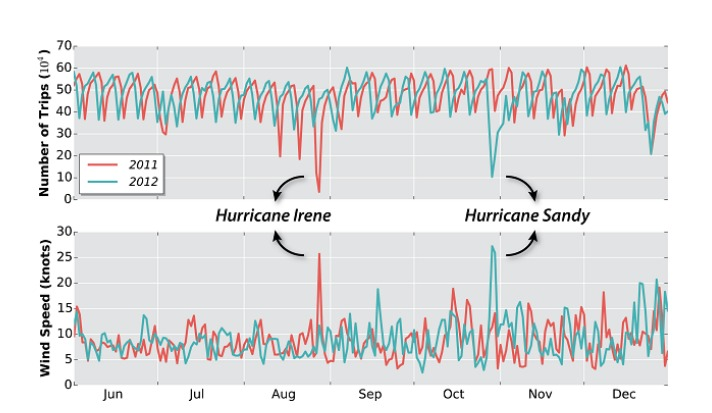
\includegraphics[width=\textwidth]{images/outlier-freire-figure-1}
% 	\caption{Figure taken from \cite{DBLP:journals/debu/FreireCVZ16} showing  relationship between the number of taxi trips over time and wind speed}
% 	\label{fig:freire-paper-taxi-wind}
% 	\vspace{-10pt}
% \end{figure*}

\begin{figure*}[t]
	\centering
	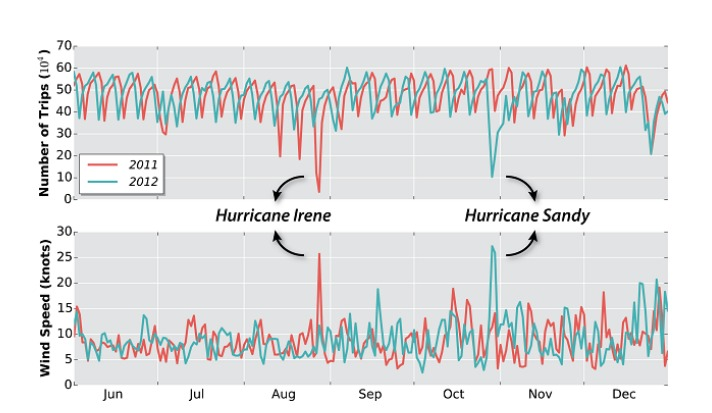
\includegraphics[width=\textwidth]{images/outlier-freire-figure-1}
	\caption{Figura tirada do \cite{DBLP:journals/debu/FreireCVZ16} mostrando a relação entre o número de corridas de táxis e a velocidade do vento}
	\label{fig:freire-paper-taxi-wind}
	\vspace{-10pt}
\end{figure*}

% \section{Context}
\section{Contextualização}

% Nowadays we are more and more connected with multiple applications that access a huge
% amount of our existing data and even generate more to improve their analyses about
% us for diverses proposals. Tools like Google Maps, Uber, Waze has a lot of realtime
% spatial data about our traffic behavior (private cars, public transportation, taxis,
% etc.), work place, travel location, etc.

Hoje em dia nós estamos mais e mais conectados com múltiplas aplicações que acessam um imenso montante dos nossos dados existentes e ainda gera mais dados para melhorar suas análises sobre nós por diversos motivos. Ferramentas como Google Maps, Uber e Waze possuem muitos dados espaciais em tempo real sobre o nosso comportamento em relação ao tráfego (carros, transporte público, táxis, etc.), local de trabalho, locais de viagem frequentes, etc.
% botar o site das ferramentas

% When it comes to regular users, it is very common that he will be lost in such masses
% of spatial data and this will damage your possible analyse, even the simplest one.
% This commom problem still does not have an definitively solution, so existing researches
% trying to indicate possible approaches for mitigate this problem and be close to a
% working solution. These approaches are based on: agroup a large amount of data by specific
% attributes and summarize the commom attributes between those data for give simple
% insights about these groups, filter the dataset to reduce the showing possibilities and
% focus on specific data for a more detailed (but not wide) analysis, and a lot of others
% strategies to reduce the complexity of the analysis.

Quando tratamos usuários comuns, é muito comum que ele se perca frente à tanta massa de dados espaciais e isso vai prejudicar sua possível análise sobre o conjunto, mesmo a mais simples. Esse problema comum ainda não tem uma solução definitiva, então pesquisas atuais tentam indicar possíveis estratégias para mitigar esse problema e se aproximar de uma solução funcional. Essas abordagens são baseada em: agrupar um grande conjunto de dados por um ou mais atributos específicos e resumir esses grupos baseado nesses atributos para conseguir simples \textit{insights} sobre esses conjuntos, filtrar o dataset para reduzir os dados visíveis e focar em dados específicos para uma análise mais precisa (mas não vasta), e muitas outras estratégias para reduzir a complexidade da análise.

% Together with those most commom problems, exists an important one that can happen before
% the first step of analysis that is: What do when parts of the dataset seems to be irregular
% or with corrupted data? There are techniques that helps to clean those parts and not compromise
% the analysis,
% % citar algum artigo sobre limpeza de dados
% but recently studies points the importance of these \textit{"abnormal"} data and how much
% the analyst can learn just studying more precisely this set. \cite{DBLP:journals/debu/FreireCVZ16}

Junto desses problemas mais comuns, existe um importante que acontece antes do primeiro passo da análise que é: \textit{O que fazer quando partes do dataset parecem irregular ou com dados corrompidos?}. Existem técnicas que ajudam na limpeza dessas partes de forma que não prejudique a análise, mas estudos recentes demonstram a importância desses dados \textit{``anormais''} e o quanto um analista pode aprender estudando mais precisamente esse conjunto \cite{DBLP:journals/debu/FreireCVZ16}.
% % citar algum artigo sobre limpeza de dados

% In this complex environment of spatial data analyses with a lot of variables and possibilities,
% an user can easily fail in some of these step compromising severely the results of his analysis.
% Combining all these details, we suggest an approach that take as relevant the user feedback
% (capturing the mouse track) and based on those feedback, we will be able to analyse the user
% interest and inside this we can detect, study and propose actions to perform when an data
% considered outlier appears in this region of user interest.

Nesse ambiente complexo de análise de dados espaciais com bastante variáveis e possibilidades, um usuário pode facilmente falhar numa dessas tarefas e comprometer seriamente o resultado de suas análises. Combinando todos esses detalhes, nós sugerimos uma abordagem que leve em consideração o \textit{feedback} do usuário (capturando o movimento do mouse) e, baseado nesse feedback, nós nos tornaremos apto a analisar o interesse do usuário e dentro disso nós podemos detectar, estudar e propor ações para serem tomadas quando um dado considerado um outlier apareça nessa região de interesse do usuário.

% \section{Objectives}
\section{Objetivos}

% In this section are defined the general and specific objectives of the work.

Nesta seção estão definidos os objetivos gerais e específicos do trabalho.

% \subsection{General Objectives}
\subsection{Objetivos Gerais}

\begin{itemize}
	% \item
	%       Introduce the problem of data analysis and visualization in large spatiotemporal
	%       datasets nowadays.
	% \item
	%       Explain our proposed approach to detect spatial outliers in large datasets using
	%       the concept of IDR and capturing user's feedback.
	% \item
	%       Present our results using the given approach to detect outliers in our spatial-temporal
	%       environment and the benefits of these experiments.
	\item
	      Introduzir o problema da análise e visualização em grandes conjuntos de dados espaço temporal atualmente.
	\item
	      Explicar nossa abordagem proposta para detecção de outliers espaciais em grandes datasets utilizando o conceito de IDR e capturando o feedback do usuário.
	\item
	      Apresentar nossos resultados utilizando a proposta para detecção de outliers no nosso ambiente espaço-temporal e os benefícios desse experimento.

\end{itemize}

% \subsection{Specific Objectives}
\subsection{Objetivos Específicos}

\begin{itemize}
	% \item
	%       Analyze the latest researches in the field of outlier detection in spatial-temporal
	%       datasets.
	\item
	      Analisar as pesquisas mais recentes na área de detecção de outliers em dados espaço-temporal.
	      % \item
	      %       Present our proposed tool for spatial-temporal data analysis and visualization.
	\item
	      Apresentar nossa ferramenta proposta para análise e visualização de dados espaço-temporal.
	\item
	      % Compare the presented researches showing the pros and cons of each work.
	      Comparar as pesquisas apresentadas destacando os prós e contras de cada pesquisa.
	\item
	      % Describe the concept of IDR used in our tool to mapping the user preference in a
	      % spatial-temporal environment.
	      Descrever o conceito de IDR utilizado na nossa ferramenta para mapear a preferência do usuário em um ambiente espaço-temporal.
	\item
	      % Summarize the most known existing outlier detection algorithms for generic and  spatial data.
	      Resumir os algoritmos de detecção de outliers mais conhecidos para dados genéricos e espaciais.
	\item
	      % Display our chosen outlier detection algorithm and explain the reasons for this choice.
	      Mostrar o nosso algoritmo escolhido explicando as razões dessa escolha.
	\item
	      % Apply our IDR concept and our chosen outlier detection algorithm in a  spatial-temporal data environment.
	      Aplicar nosso conceito de IDR e nosso algoritmo de detecção de outlier escolhido num ambiente de dados espaço-temporal.
	\item
	      % Present the results of our application and indicate our future work.
	      Apresentar os resultados de nossa aplicação e indicar nossos trabalhos futuros.

\end{itemize}

% \section{Work Organization}
\section{Organização do Trabalho}

% The document is organized as follows. Section 2 summaries the existing researches
% in data analysis and visualization field comparing with our proposed tool. Section 3 describes
% the concepts of IDRs (Interesting Dense Region) and Outliers with the existing algorithms for
% their detection and our chosen algorithm to detect outliers in our platform. Section 4 explains
% how we apply the IDRs and outliers detection in the GeoGuide tool. Section 5 presents two
% applications using distinct datasets to demonstrate the applicability of it to real-world
% problems and the advantages of this approach. It shows and discusses the outlier detection
% results. Finally, a conclusion and some directions for future works are given in Section 6.

O documento é organizado do seguinte modo: Seção 2 resume as pesquisas existentes no campo da análise e visualização de dados comparando com nossa ferramenta proposta. Seção 3 descreve os conceitos de IDRs (\textit{Interesting Dense Region}) e Outliers com os algoritmos existentes para sua detecção e nosso algoritmo escolhido para detectar outliers em nossa plataforma. Seção 4 explica como aplicamos as IDRs e detecção de outliers na ferramenta GeoGuide. Seção 5 apresenta duas aplicações utilizando datasets distintos para demonstrar a aplicabilidade disso em problemas do mundo real e as vantagens dessa abordagem, mostrando e discutindo os resultados da detecção de outliers. Por fim, a conclusão e algumas direções para trabalhos futuros são dados na Seção 6.